\documentclass{article}
\setlength{\parskip}{5pt} % esp. entre parrafos
\setlength{\parindent}{0pt} % esp. al inicio de un parrafo
\usepackage{listings} % listings
\usepackage{color} %colores
\usepackage{amsmath} % mates
\usepackage[sort&compress,numbers]{natbib} % referencias
\usepackage{url} % que las URLs se vean lindos
\usepackage[top=15mm,left=20mm,right=20mm,bottom=25mm]{geometry} % margenes
\usepackage{hyperref} % ligas de URLs
\usepackage{graphicx} % poner figuras
\usepackage[spanish]{babel} % otros idiomas

\author{Claudia Lizeth Hern\'andez Ram\'irez} % author
\title{Homework 3 - Teoría de Colas} % titulo
\date{\today}

\definecolor{mypink}{rgb}{0.976, 0.462, 0.847}
\definecolor{mygray}{rgb}{0.976, 0.980, 0.980}
\definecolor{myblue}{rgb}{0.258, 0.682, 1}
\definecolor{mypink2}{rgb}{0.525, 0.054, 0.4}
\lstset{ 
  backgroundcolor=\color{mygray},
  commentstyle=\color{myblue},
  keywordstyle=\color{mypink}, 
  numberstyle=\tiny\color{mypink}
  stringstyle=\color{mypink2}, 
  breaklines=true,
}


\begin{document} % inicia contenido

\maketitle % cabecera

% RESUMEEEEEEEEEEEEEEEN
\begin{abstract} % resumen
  \centering
En mayor\'ia, las diferencias en las medianas son estad\'isticamente significativas.
  
\end{abstract}


% INTRODUCCIOOOOOOOOOOOON
\section{Introducci\'{o}n}\label{intro} % seccion y etiqueta
En esta tarea se pretende determinar la cambio que presenta el tiempo de realizaci\'on de una tarea con respecto a la variac\'on de los n\'ucleos de trabajo y el orden con que se realizan las tareas.



% DESARROLLOOOOOOOOOOOO
\section{Desarrollo}\label{desarrollo} % Desarrollo de la tarea
Comenzamos generando n\'umeros primo utilizando el código que se nos proporcion\'o en clase \cite{RepoDraElisa}.\; Una vez obtenidos los datos, los export\'e a una archivo \texttt{.xlsx} para visualizarlos de una mejor manera.


\begin{lstlisting}[language=Python, caption= C\'odigo para generar n\'umeros primo.]

from time import time
from math import sqrt, ceil
from random import randint, random, shuffle

def primo(n):
    if n < 4: # 1 2 3
        return True
    if n % 2 == 0:
        return False
    for d in range(3, int(ceil(sqrt(n)))):
        if n % d == 0:
            return False
    return True

dificiles = []
meta = 10
faciles = [randint(1000, 15000) for i in range(meta)]
while len(dificiles) < meta:
    n = randint(50000000, 100000000) 
    if n % 2 == 0:
        n += 1
    if primo(n):
        dificiles.append(n)

from multiprocessing import Pool

if __name__ == "__main__":
    c1 = faciles + dificiles
    c2 = dificiles + faciles
    cr = c2.copy()
    shuffle(cr)
    ordenes = {'fp': c1, 'dp': c2, 'oa': cr}
    for trabajadores in range(1, 5):
        with Pool(trabajadores) as p:
            for o in ordenes:
                label = o
                datos = ordenes[o]
                for replica in range(10):
                    start = time()
                    p.map(primo, datos)
                    tiempo = 1000 * (time() - start)
                    if replica > 0:
                        print(f'{replica},{trabajadores},{label},{tiempo}')
\end{lstlisting}


Posteriormente en \texttt{RStudio} gener\'e un \texttt{data.frame} en donde est\'an representados el \texttt{n\'umero de trabajadores} como \texttt{NDT}, el \texttt{tipo de trabajo} como \texttt{TDT} y el \texttt{tiempo} como \texttt{Tiempo}.
Teniendo el data frame, gener\'e una gr\'afica de caja-bigote.
\begin{figure}[h!] % figura
    \centering
    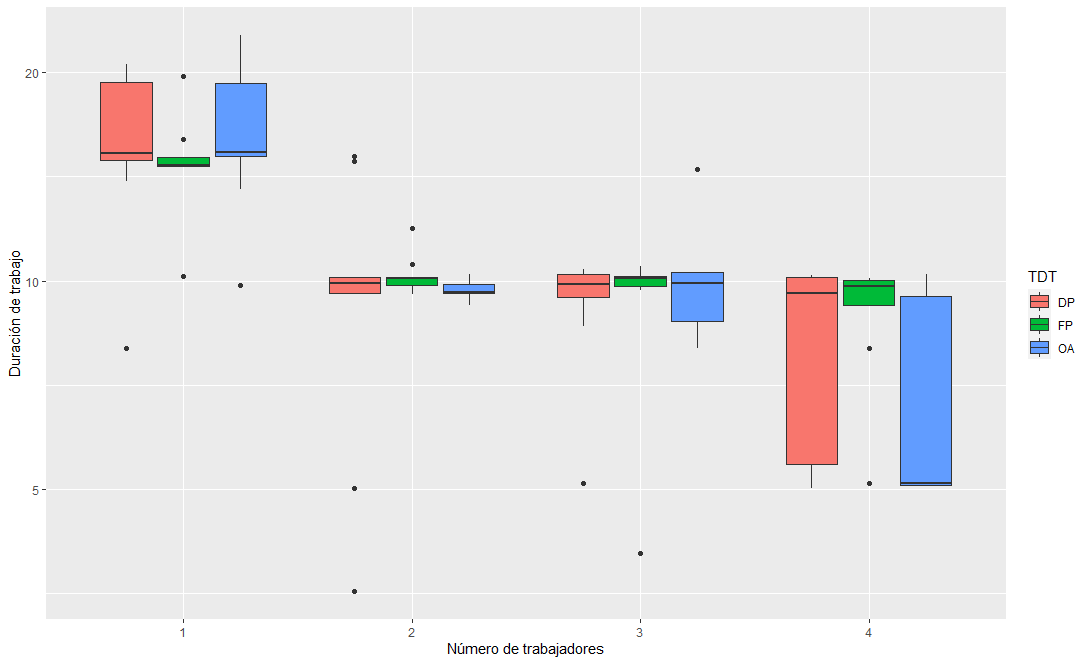
\includegraphics[width=150mm]{Boxplot.JPG} % archivo
    \caption{Variaci\'on del tiempo con respecto al TDT (Tipo de tarea) y la Cantidad de n\'ucleos ejecutando la tarea.}
    \label{Figura 1}
\end{figure}

Apliqu\'e pruebas de normalidad a mis datos para determinar con  qu\'e prueba estad\'istica trabajar\'ia.
Pod\'ia utlizar \texttt{Kolmogorov Smirnov} sin embargo, al tener muestran tan pequeñas no resultaba conveniente utilizarla, por lo que opt\'e por emplear la prueba de normalidad de \texttt{Shapiro Wilk} \cite{PruebasNormalidad}.

\begin{table}[ht]
    \centering
    \caption{Resultados obtenidos de prueba de normalidad de Shapiro - Orden de tareas.} 
    \begin{tabular}{|c|c|c|}
    \hline
    DDT & W & P  \\
    \hline
    DPP & 0.9389 & 0.0472 \\
    \hline
    FPP & 0.8448 & 0.0001 \\
    \hline
    OAA & 0.9307 & 0.0264\\
    \hline
\end{tabular}
    \label{cuadro 1}
\end{table}

\begin{table}[ht]
    \centering
    \caption{Resultados obtenidos de prueba de normalidad de Shapiro - N\'ucleos.} 
    \begin{tabular}{|c|c|c|}
    \hline
    N\'ucleos & W & P  \\
    \hline
    1 & 0.9221 & 0.0445 \\
    \hline
    2 & 0.0.7207 & 0.0000 \\
    \hline
    3 & 0.0.7193 & 0.0000 \\
    \hline
    4 & 0.7918 & 0.0000 \\
    \hline
\end{tabular}
    \label{cuadro 2}
\end{table}

- \texttt{Hip\'otesis nula}: la distancia de la variable es normal.

- \texttt{Hip\'otesis alternativa}: la distribuci\'on de la variable no es normal.

En la literatura podemos encontrar que diversos autores establecen que para pruebas de normalidad que para aceptar la hip\'otesis nula el valor de \texttt{P} debe ser mayor al 0.05, es decir mayor al 5\%. De los resultados mostrados en el cuadro 1 podemos deducir ya que nuestros valores de \texttt{P} son menores a 0.05, que nuestra hip\'otesis nula es \texttt{rechazada}.

Con esta informaci\'on podemos comenzar a decidir qu\'e prueba estad\'istica utilizaremos para desarrollar nuestra tarea.
Queda claro que la distribuci\'on de nuestros datos no es normal, tenemos m\'as de dos grupos a analizar y son muestras independientes, por lo que resulta conveniente utilizar  la prueba de \texttt{Kruskal-Wallis}\cite{SeleccionPruebas}.Para comenzar a trabajar con mi prueba de Kruskal-Wallis gener\'e diversos vectores que me ayudar\'ian a hacer el an\'alisis. 

\begin{table}[ht]
    \centering
    \caption{Resultados obtenidos de prueba Kruskal-Wallis - Orden de tareas.} 
    \begin{tabular}{|c|c|c|c|}
    \hline
    Tareas & Chi cuadrada & DF & P  \\
    \hline
    Dif\'iciles primero 4 n\'ucleos & 13.933 & 3 & 0.002997 \\
    \hline
    F\'aciles primero 4 n\'ucleos & 20.269 & 3 & 0.000149 \\
    \hline
    Aleatorias 4 n\'ucleos & 19.088 & 3 & 0.000262\\
    \hline
\end{tabular}
    \label{cuadro 3}
\end{table}
\begin{table}[ht]
    \centering
    \caption{Resultados obtenidos de prueba Kruskal-Wallis - N\'ucleos} 
    \begin{tabular}{|c|c|c|c|}
    \hline
    N\'ucleos & Chi cuadrada & DF & P  \\
    \hline
    1 & 2.2011 & 2 & 0.3327 \\
    \hline
    2 & 1.8025 & 2 & 0.4061 \\
    \hline
    3 & 1.1478 & 2 & 0.5633 \\
    \hline
    4 & 1.3173 & 2 & 0.5175 \\
    \hline
\end{tabular}
    \label{cuadro 4}
\end{table}


A continuaci\'on se muestra el c\'odigo final.

\begin{lstlisting}[language=R, caption= C\'odigo utilizado para generar Boxplot.]
library(ggplot2)
library(scales)
library(tidyverse)

datos = data.frame(
  "NDT" = rep(c(1, 2, 3, 4), times = c(27, 27, 27, 27)), #repite del al 4 27 veces cada uno
  "TDT" = rep(c("FP", "DP", "OA", "FP", "DP", "OA", "FP", "DP", "OA", "FP", "DP", "OA"), times = c(9, 9, 9, 9, 9, 9, 9, 9, 9, 9, 9, 9)), 
  "Tiempo" = c(14.6632194519042,	14.6689414978027,	14.6400928497314,	14.7817134857177,	10.1368427276611,	16.0033702850341,	15.1014328002929,	14.5940780639648,	19.763708114624,	15.0637626647949,	8.00037384033203,	20.5345153808593,	14.9371623992919,	15.2616500854492,	15.5577659606933,	13.9107704162597,	19.8197364807128,	19.3409919738769,	20.5903053283691,	17.2526836395263,	9.84764099121093,	15.1457786560058,	15.122652053833,	15.3250694274902,	19.301414489746,	22.6647853851318,	13.5760307312011,	9.5534324645996,	10.1165771484375,	10.5707645416259,	10.1063251495361,	10.0808143615722,	9.58919525146484,	9.85145568847656,	11.9268894195556,	9.95707511901855,	9.93013381958007,	3.55696678161621,	9.91225242614746,	10.1029872894287,	9.59086418151855,	10.1222991943359,	14.8596763610839,	15.1095390319824,	5.00893592834472,	9.58704948425292,	10.1697444915771,	10.23530960083,	9.61017608642578,	9.20867919921875,	9.60993766784667,	9.87768173217773,	9.60707664489746,	9.50002670288085,	10.0886821746826,	10.1439952850341,	10.5109214782714,	4.04214859008789,	10.0753307342529,	9.83428955078125,	9.97304916381835,	10.3750228881835,	9.69386100769042,	0,	9.85026359558105,	10.1709365844726,	9.75704193115234,	9.92989540100097,	10.394811630249,	10.3027820587158,	8.60190391540527,	5.08999824523925,	7.99918174743652,	9.51886177062988,	0,	10.2787017822265,	10.3039741516113,	8.00061225891113,	14.5168304443359,	9.90939140319824,	0,	9.6750259399414,	10.0939273834228,	5.09929656982421,	9.71102714538574,	9.9799633026123,	10.0970268249511,	0,	8.00085067749023,	9.92918014526367,	9.59515571594238,	5.56445121765136,	5.07974624633789,	10.1842880249023,	9.59181785583496,	0,	5.00750541687011,	10.0986957550048,	10.1239681243896,	5.04970550537109,	10.1282596588134,	5.0969123840332,	5.04279136657714,	10.2267265319824,	5.08332252502441,	5.0661563873291,	9.28521156311035,	0)
)
datos 

datos$NDT = as.factor(datos$NDT)
datos$TDT = as.factor(datos$TDT)

ggplot(datos, aes(x = NDT, y = Tiempo, fill = TDT)) +
  geom_boxplot() +
  scale_y_log10() +
  labs( x = "Número de trabajadores", y = "Duración de trabajo")
\end{lstlisting}


\begin{lstlisting} [language=R, caption= C\'odigo utilizado para hacer pruebas de normalidad seg\'un los n\'ucleos que estan trabajando.]
DPS = data_frame(
  NDTT = rep(c(1, 2, 3, 4), times = c(9, 9, 9, 9)), 
  "DPP" = c(15.0637626647949,	8.00037384033203,	20.5345153808593,	14.9371623992919,	15.2616500854492,	15.5577659606933,	13.9107704162597,	19.8197364807128,	19.3409919738769, 9.93013381958007,	3.55696678161621,	9.91225242614746,	10.1029872894287,	9.59086418151855,	10.1222991943359,	14.8596763610839,	15.1095390319824,	5.00893592834472, 0,	9.85026359558105,	10.1709365844726,	9.75704193115234,	9.92989540100097,	10.394811630249,	10.3027820587158,	8.60190391540527,	5.08999824523925, 9.59515571594238,	5.56445121765136,	5.07974624633789,	10.1842880249023,	9.59181785583496,	0,	5.00750541687011,	10.0986957550048,	10.1239681243896)
)
shapiro.test(DPS$DPP)


FPS = data_frame(
  NDTT = rep(c(1, 2, 3, 4), times = c(9, 9, 9, 9)), 
  "FPP" = c(14.6632194519042,	14.6689414978027,	14.6400928497314,	14.7817134857177,	10.1368427276611,	16.0033702850341,	15.1014328002929,	14.5940780639648,	19.763708114624, 9.5534324645996,	10.1165771484375,	10.5707645416259,	10.1063251495361,	10.0808143615722,	9.58919525146484,	9.85145568847656,	11.9268894195556,	9.95707511901855, 10.0886821746826,	10.1439952850341,	10.5109214782714,	4.04214859008789,	10.0753307342529,	9.83428955078125,	9.97304916381835,	10.3750228881835,	9.69386100769042, 9.6750259399414,	10.0939273834228,	5.09929656982421,	9.71102714538574,	9.9799633026123,	10.0970268249511,	0,	8.00085067749023,	9.92918014526367)
)
shapiro.test(FPS$FPP)


OAS = data_frame(
  NDTT = rep(c(1, 2, 3, 4), times = c(9, 9, 9, 9)), 
  "OAA" = c(20.5903053283691,	17.2526836395263,	9.84764099121093,	15.1457786560058,	15.122652053833,	15.3250694274902,	19.301414489746,	22.6647853851318,	13.5760307312011, 9.58704948425292,	10.1697444915771,	10.23530960083,	9.61017608642578,	9.20867919921875,	9.60993766784667,	9.87768173217773,	9.60707664489746,	9.50002670288085, 7.99918174743652,	9.51886177062988,	0,	10.2787017822265,	10.3039741516113,	8.00061225891113,	14.5168304443359,	9.90939140319824,	0, 5.04970550537109,	10.1282596588134,	5.0969123840332,	5.04279136657714,	10.2267265319824,	5.08332252502441,	5.0661563873291,	9.28521156311035,	0)
)
shapiro.test(OAS$OAA)
\end{lstlisting}


\begin{lstlisting}[language=R, caption= C\'odigo utilizado para hacer pruebas de normalidad seg\'un el orden en que se ejecutan las tareas.]
NDT1 = data.frame(
  TDTT = rep(c("FP", "DP", "OA"), times = c(9, 9, 9)),
  "NDTS1" = c(14.6632194519042, 	14.6689414978027, 	14.6400928497314, 	14.7817134857177, 	10.1368427276611, 	16.0033702850341, 	15.1014328002929, 	14.5940780639648, 	19.763708114624, 	15.0637626647949, 	8.00037384033203, 	20.5345153808593, 	14.9371623992919, 	15.2616500854492, 	15.5577659606933, 	13.9107704162597, 	19.8197364807128, 	19.3409919738769, 	20.5903053283691, 	17.2526836395263, 	9.84764099121093, 	15.1457786560058, 	15.122652053833, 	15.3250694274902, 	19.301414489746, 	22.6647853851318, 	13.5760307312011)
)
shapiro.test(NDT1$NDTS1)

NDT2 = data_frame(
  TDTT = rep(c("FP", "DP", "OA"), times = c(9, 9, 9)),
  "NDTS2" = c(9.5534324645996, 	10.1165771484375, 	10.5707645416259, 	10.1063251495361, 	10.0808143615722, 	9.58919525146484, 	9.85145568847656, 	11.9268894195556, 	9.95707511901855, 	9.93013381958007, 	3.55696678161621, 	9.91225242614746, 	10.1029872894287, 	9.59086418151855, 	10.1222991943359, 	14.8596763610839, 	15.1095390319824, 	5.00893592834472, 	9.58704948425292, 	10.1697444915771, 	10.23530960083, 	9.61017608642578, 	9.20867919921875, 	9.60993766784667, 	9.87768173217773, 	9.60707664489746, 	9.50002670288085)
)
shapiro.test(NDT2$NDTS2)

NDT3 = data_frame(
  TDTT = rep(c("FP", "DP", "OA"), times = c(9, 9, 9)),
  "NDTS3" = c(10.0886821746826, 	10.1439952850341, 	10.5109214782714, 	4.04214859008789, 	10.0753307342529, 	9.83428955078125, 	9.97304916381835, 	10.3750228881835, 	9.69386100769042, 	0, 	9.85026359558105, 	10.1709365844726, 	9.75704193115234, 	9.92989540100097, 	10.394811630249, 	10.3027820587158, 	8.60190391540527, 	5.08999824523925, 	7.99918174743652, 	9.51886177062988, 	0, 	10.2787017822265, 	10.3039741516113, 	8.00061225891113, 	14.5168304443359, 	9.90939140319824, 	0)
)
shapiro.test(NDT3$NDTS3)

NDT4 = data_frame(
  TDTT = rep(c("FP", "DP", "OA"), times = c(9, 9, 9)),
  "NDTS4" = c(9.6750259399414, 	10.0939273834228, 	5.09929656982421, 	9.71102714538574, 	9.9799633026123, 	10.0970268249511, 	0, 	8.00085067749023, 	9.92918014526367, 	9.59515571594238, 	5.56445121765136, 	5.07974624633789, 	10.1842880249023, 	9.59181785583496, 	0, 	5.00750541687011, 	10.0986957550048, 	10.1239681243896, 	5.04970550537109, 	10.1282596588134, 	5.0969123840332, 	5.04279136657714, 	10.2267265319824, 	5.08332252502441, 	5.0661563873291, 	9.28521156311035, 	0)
)
shapiro.test(NDT4$NDTS4)
\end{lstlisting}


\begin{lstlisting}[language=R, caption= C\'odigo utilizado para hacer pruebas de Kurskal-Wallis (N\'ucleos).]
DP1 = c(15.0637626647949,	8.00037384033203,	20.5345153808593,	14.9371623992919,	15.2616500854492,	15.5577659606933,	13.9107704162597,	19.8197364807128,	19.3409919738769)
DP2 = c(9.93013381958007,	3.55696678161621,	9.91225242614746,	10.1029872894287,	9.59086418151855,	10.1222991943359,	14.8596763610839,	15.1095390319824,	5.00893592834472)
DP3 = c(0,	9.85026359558105,	10.1709365844726,	9.75704193115234,	9.92989540100097,	10.394811630249,	10.3027820587158,	8.60190391540527,	5.08999824523925)
DP4 = c(9.59515571594238,	5.56445121765136,	5.07974624633789,	10.1842880249023,	9.59181785583496,	0,	5.00750541687011,	10.0986957550048,	10.1239681243896)
kruskal.test(list(DP1, DP2, DP3, DP4))

FP1= c(14.6632194519042,	14.6689414978027,	14.6400928497314,	14.7817134857177,	10.1368427276611,	16.0033702850341,	15.1014328002929,	14.5940780639648,	19.763708114624)
FP2= c(9.5534324645996,	10.1165771484375,	10.5707645416259,	10.1063251495361,	10.0808143615722,	9.58919525146484,	9.85145568847656,	11.9268894195556,	9.95707511901855)
FP3= c(10.0886821746826,	10.1439952850341,	10.5109214782714,	4.04214859008789,	10.0753307342529,	9.83428955078125,	9.97304916381835,	10.3750228881835,	9.69386100769042)
FP4= c(9.6750259399414,	10.0939273834228,	5.09929656982421,	9.71102714538574,	9.9799633026123,	10.0970268249511,	0,	8.00085067749023,	9.92918014526367)
kruskal.test(list(FP1, FP2, FP3, FP4))

OA1 = c(20.5903053283691,	17.2526836395263,	9.84764099121093,	15.1457786560058,	15.122652053833,	15.3250694274902,	19.301414489746,	22.6647853851318,	13.5760307312011)
OA2 = c(9.58704948425292,	10.1697444915771,	10.23530960083,	9.61017608642578,	9.20867919921875,	9.60993766784667,	9.87768173217773,	9.60707664489746,	9.50002670288085)
OA3 = c(7.99918174743652,	9.51886177062988,	0,	10.2787017822265,	10.3039741516113,	8.00061225891113,	14.5168304443359,	9.90939140319824,	0)
OA4 = c(5.04970550537109,	10.1282596588134,	5.0969123840332,	5.04279136657714,	10.2267265319824,	5.08332252502441,	5.0661563873291,	9.28521156311035,	0)
kruskal.test(list(OA1, OA2, OA3, OA4))
\end{lstlisting}


\begin{lstlisting}[language=R, caption= C\'odigo utilizado para hacer pruebas de Kurskal-Wallis (Orden Tareas).]
NDT1FP = c (14.6632194519042,	14.6689414978027,	14.6400928497314,	14.7817134857177,	10.1368427276611,	16.0033702850341,	15.1014328002929,	14.5940780639648,	19.763708114624)
NDT1DP = c (15.0637626647949,	8.00037384033203,	20.5345153808593,	14.9371623992919,	15.2616500854492,	15.5577659606933,	13.9107704162597,	19.8197364807128,	19.3409919738769)
NDT1OA = c(20.5903053283691,	17.2526836395263,	9.84764099121093,	15.1457786560058,	15.122652053833,	15.3250694274902,	19.301414489746,	22.6647853851318,	13.5760307312011)
kruskal.test(list(NDT1FP, NDT1DP, NDT1OA))

NDT2FP = c(9.5534324645996,	10.1165771484375,	10.5707645416259,	10.1063251495361,	10.0808143615722,	9.58919525146484,	9.85145568847656,	11.9268894195556,	9.95707511901855)
NDT2DP = c(9.93013381958007,	3.55696678161621,	9.91225242614746,	10.1029872894287,	9.59086418151855,	10.1222991943359,	14.8596763610839,	15.1095390319824,	5.00893592834472)
NDT2OA = c(9.58704948425292,	10.1697444915771,	10.23530960083,	9.61017608642578,	9.20867919921875,	9.60993766784667,	9.87768173217773,	9.60707664489746,	9.50002670288085)
kruskal.test(list(NDT2FP, NDT2DP, NDT2OA))

NDT3FP = c(10.0886821746826,	10.1439952850341,	10.5109214782714,	4.04214859008789,	10.0753307342529,	9.83428955078125,	9.97304916381835,	10.3750228881835,	9.69386100769042)
NDT3DP = c(0,	9.85026359558105,	10.1709365844726,	9.75704193115234,	9.92989540100097,	10.394811630249,	10.3027820587158,	8.60190391540527,	5.08999824523925)
NDT3OA = c(7.99918174743652,	9.51886177062988,	0,	10.2787017822265,	10.3039741516113,	8.00061225891113,	14.5168304443359,	9.90939140319824,	0)
kruskal.test(list(NDT3FP, NDT3DP, NDT3OA))

NDT4FP = c(9.6750259399414,	10.0939273834228,	5.09929656982421,	9.71102714538574,	9.9799633026123,	10.0970268249511,	0,	8.00085067749023,	9.92918014526367)
NDT4DP = c(9.59515571594238,	5.56445121765136,	5.07974624633789,	10.1842880249023,	9.59181785583496,	0,	5.00750541687011,	10.0986957550048,	10.1239681243896)
NDT4OA = c(5.04970550537109,	10.1282596588134,	5.0969123840332,	5.04279136657714,	10.2267265319824,	5.08332252502441,	5.0661563873291,	9.28521156311035,	0)
kruskal.test(list(NDT4FP, NDT4DP, NDT4OA))
\end{lstlisting}

Uso listings \cite{CalculatorColor, Listingscolor, ListingsWidth}.

%CONCLUSIOOOON
\section{Conclusi\'on}
Teniendo que:

-Hip\'otesis nula: las medias de poblaci\'on son todas iguales.

-Hip\'otesis alternativa: las medias de poblaci\'on no son todas iguales.
y con un nivel de significancia = 0.05 podemos crechazar la hip\'otesis nula, por lo tanto las diferencias entre algunas medianas son estad\'isticamente significativas. Sin embargo podemos observar que para el an\'alisis de 3 y 4 n\'ucleos podemos aceptar la hip\'otesis nula y decir que en esos valores, las diferencias en las medianas no son significativas.

% BIBLIOGRAFIAAAAAAS
\bibliography{referencias}
\bibliographystyle{plainnat}
\end{document}

